\chapter{Design \& Implementation}
The project experimented with Flutter for the initial simulation due to the benefits of pixel-level control and fast prototyping (see Figure \ref{fig:first-waves} for a preview of the first successful waves). However, the rendering was too slow for large chemical circuits, so the GPU was needed, for which, as of March 2024 Flutter still has no official support. A custom version of the newest engine was tested to expose experimental GPU APIs as detailed in \href{flutter.dev/go/impeller-dart}{flutter.dev/go/impeller-dart}.
That did not work, so the Metal library was used to compute the simulation on the GPU. 
The Metal library is a low-level, high-performance API for the GPU, and it was chosen for its ability to run on Apple devices, which are widely used in the scientific community, the execution graph for the simulation is illustrated in Figure \ref{fig:metal-dependency-pipline}.

\begin{figure}
    \centering
    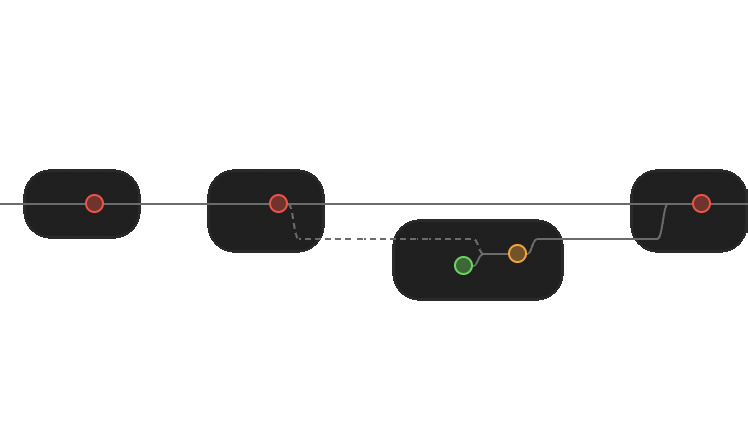
\includegraphics[width=0.5\linewidth]{metal-pipeline.png}
    \caption{The Metal Dependency Pipeline consists of a Compute Command Encoder (represented by red circles) and a Render Command Encoder (depicted by yellow circles). The Compute Command Encoder is run multiple times, performing as many calculations as possible. Simultaneously, the Render Command Encoder operates periodically to render the computed results. These two encoders work in parallel, with the Render Command Encoder producing output every time it gets a chance, while the Compute Command Encoder continuously performs computations most of the time.}
    \label{fig:metal-dependency-pipline}
\end{figure}


The mathematical principles in the Oregonator model are described in section\ref{sec:oregonator-math}.
The parameters for the simulation are listed under table\ref{tab:simulation-parameters}. 
They are standard values widely used in the literature that experiments with the Oregonator model.



\begin{table}[H]
    \centering
    \begin{tabularx}{\textwidth}{|X|X|} 
        \hline
    \textbf{Parameter} & \textbf{Value} \\ \hline
    $\epsilon$         & 0.0243         \\
    $f$                & 1.4            \\ 
    $\phi_{\text{active}}$ & 0.054          \\ 
    $\phi_{\text{passive}}$ & 0.0975          \\
    $q$                & 0.002          \\ 
    $D_u$              & 0.45           \\ 
    $\Delta t$         & 0.001          \\
    $\Delta x$              & 0.25           \\
    \hline
    \end{tabularx}
    \caption{Simulation parameters with their respective values.}
    \label{tab:simulation-parameters}
\end{table}
